\providecommand{\main}{..}
\documentclass[\main/main.tex]{subfiles}

\begin{document}
\graphicspath{{img/}{04_hardware/img/}}
\setlength{\abovecaptionskip}{0pt}
\setlength{\belowcaptionskip}{0pt}

\chapter{Anchor hardware implementation}
In this chapter, the hardware problems relating to the anchor are discussed. The chapter starts by a brief introduction to the DWM1001 module - the main hardware for this thesis. The following sections analyze some important blocks of the circuitry for an anchor proposed by this thesis. A full Altium design for the anchor is provided in appendix \ref{appendix:rtls_anchor_board}.

\section{Introduction to DWM1001 module}
\begin{figure}[H]
    \begin{center}
        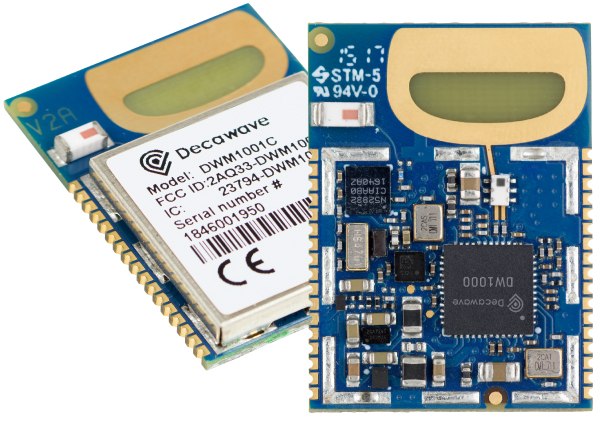
\includegraphics[width=0.3\textwidth]{DWM1001-Module_ProdPage_600x430.jpg}
    \end{center}
    \caption{DWM1001 Module}
    \label{fig:dwm1001c_module}
\end{figure}

The DWM1001 module is based on Decawave's DW1000 Ultra
Wideband (UWB) transceiver IC, which is an IEEE 802.15.4-
2011 UWB implementation. It integrates UWB and Bluetooth
antenna, all RF circuitry, Nordic Semiconductor nRF52832 and
a motion sensor.

There are multiple reasons for answering the question: why DWM1001 module is used for this thesis.
Followings are some key features:
\begin{itemize}
    \item Ranging accuracy to within 10cm
    \item UWB Channel 5 printed PCB antenna (6.5 GHz)
    \item 6.8 Mbps data rate IEEE 802.15.4-2011 UWB compliant
    \item Well known Nordic Semiconductor nRF52832 SoC
    \item Bluetooth connectivity and Bluetooth chip antenna
    \item Motion sensor is available: 3-axis accelerometer
    \item Current consumption optimized for low power sleep mode: $<$ 15$\mu$A
    \item Low supply voltage: 2.8 V to 3.6 V
    \item Small size: 19.1 mm x 26.2 mm x 2.6 mm
    \item Modules marked DWM1001C are certified to ETSI, FCC and ISED regulations
\end{itemize}

\begin{figure}[H]
    \begin{center}
        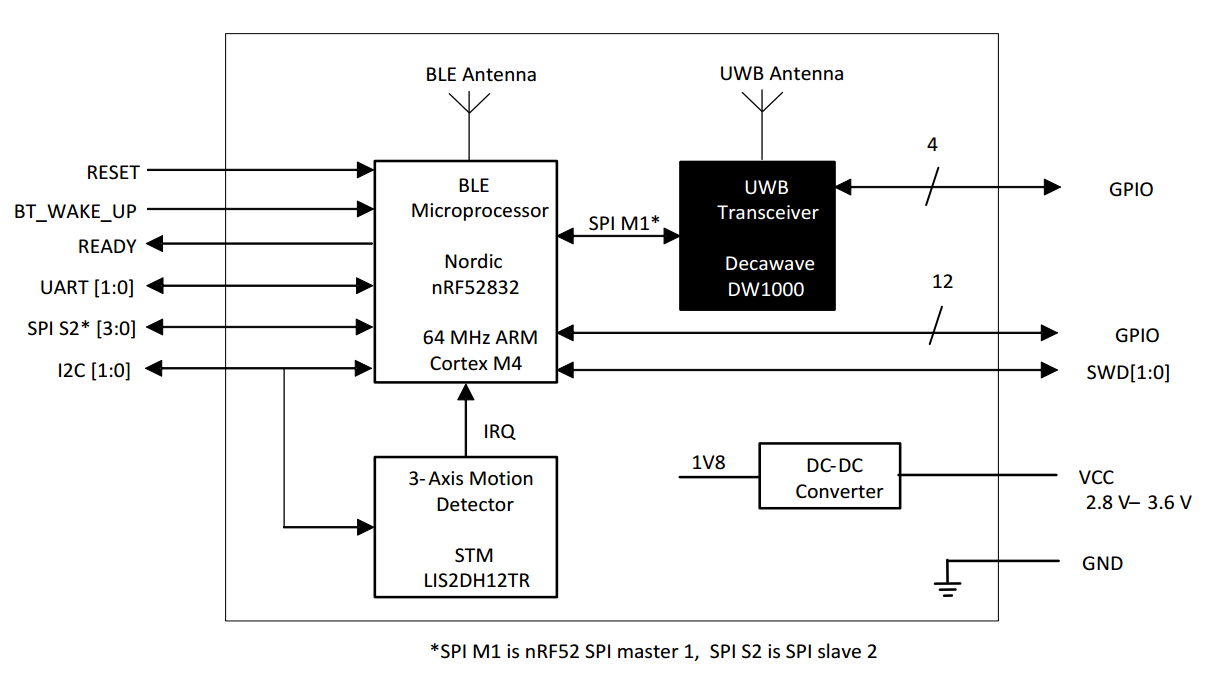
\includegraphics[scale=0.3]{dwm1001_block_diagram.png}
    \end{center}
    \caption{DWM1001 block diagram}
    \label{fig:dwm1001_block_diagram}
\end{figure}

The nRF52832 is a general-purpose multi-protocol SoC. It meets the challenges of a broad range of applications that need advanced Bluetooth LE features. It is built around an Arm® Cortex™-M4 CPU with floating-point unit running at 64 MHz. As shown in figure \ref{fig:dwm1001_block_diagram}, in the DWM1001 module, there is an nRF52832 MCU communicating to  a DW1000 radio IC over an SPI connection.

\section{Battery charger circuit}
The schematic for battery charger circuit is given in figure \ref{fig:battery_charger_circuit}. Subsequence subsections provide principle descriptions about main components of the circuit.
\begin{figure}[H]
    \begin{center}
        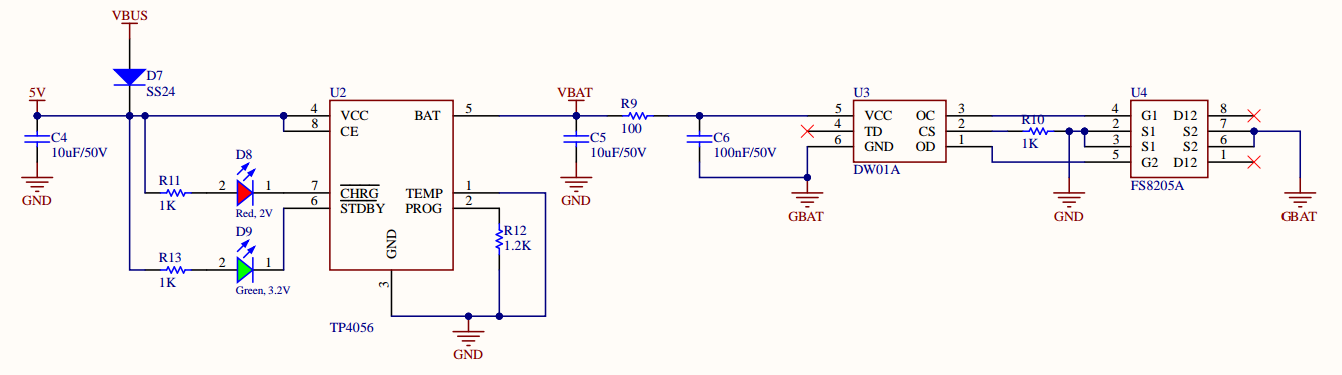
\includegraphics[width=1\textwidth]{battery_charger_circuit.png}
    \end{center}
    \caption{Battery charger circuit}
    \label{fig:battery_charger_circuit}
\end{figure}

\subsection{Constant current - constant voltage charging}

\subsubsection{CC-CV charging method}
The constant current - constant voltage (CC-CV) charging method has been extensively used for charging batteries cause it combines the advantages of both the CC and CV charging methods. As presented in figure \ref{fig:tp4056_cc_cv_profile}, the CC-CV charging method uses CC charging in the first charging stage, and when the voltage reaches the maximum safe threshold value, the charging process shifts to the CV charging method. The charging process is complete when the current levels off or when full battery capacity is reached.

\begin{figure}[H]
    \begin{center}
        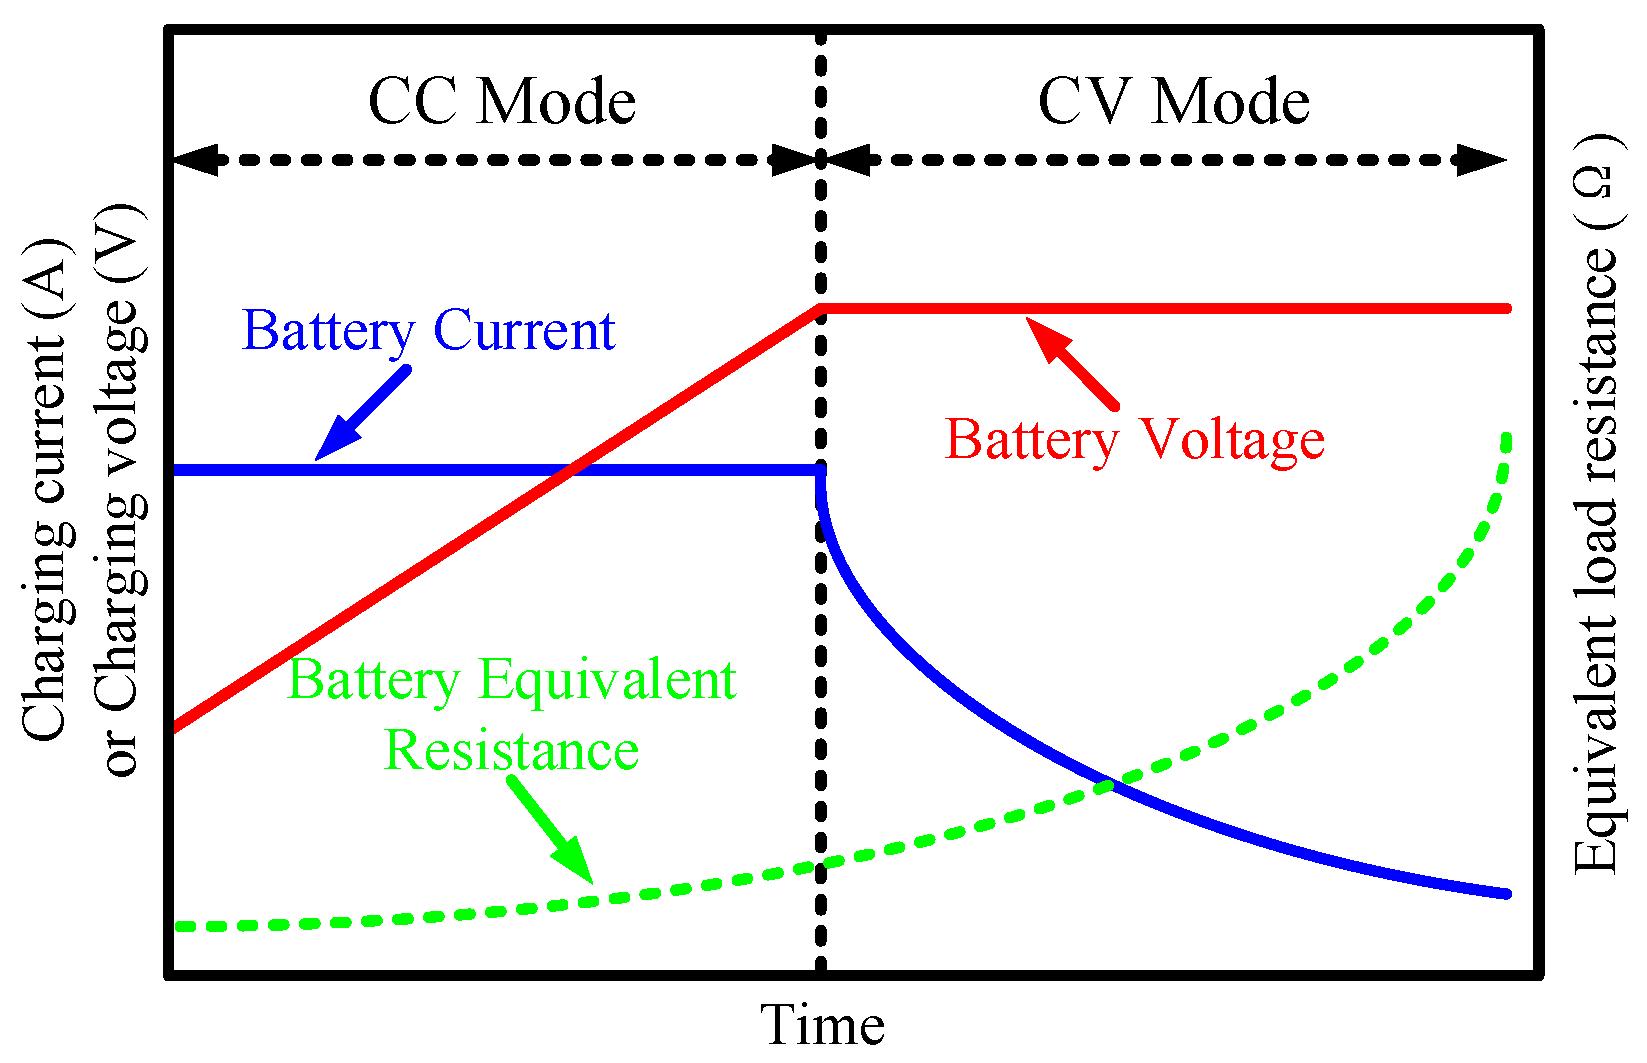
\includegraphics[width=0.6\textwidth]{tp4056_cc_cv_profile.png}
    \end{center}
    \caption{Constant current/constant voltage (CC/CV) charging profile}
    \label{fig:tp4056_cc_cv_profile}
\end{figure}

\subsubsection{CC-CV in action}
The TP4056 is a CC-CV linear charger for single-cell lithium-ion batteries. Its SOP package and low external component count make the TP4056 ideally suited for portable applications. Using TP4056, no blocking diode is required since the internal PMOSFET architecture has prevented to negative charge current circuit. The charge voltage is
fixed at 4.2V, and the charge current can be programmed externally with a single resistor. The TP4056 automatically terminates the charge cycle when the charge current drops to 1/10th the programmed value after the final float voltage is reached. 

In this thesis, the TEMP pin (Pin 1) is grounded to disabled the temperature sense function. The charge current, however, is set by connecting a resistor $R_{PROG}$ from the PROG pin (Pin 2) to GND. In this thesis, a 1.2K resistor is used for charge current setting:

\begin{equation}
    I_{BAT} = \frac{V_{PROC}}{R_{PROG}}\times 1200 = \frac{1V}{1.2K}\times 1200 = 1A
\end{equation}

Figure \ref{fig:tp4056_complete_charge_cycle} is the real profile of CC-CV charging method in the TP4056 compared to the theory profile shown in figure \ref{fig:tp4056_cc_cv_profile}.

\begin{figure}[H]
    \begin{center}
        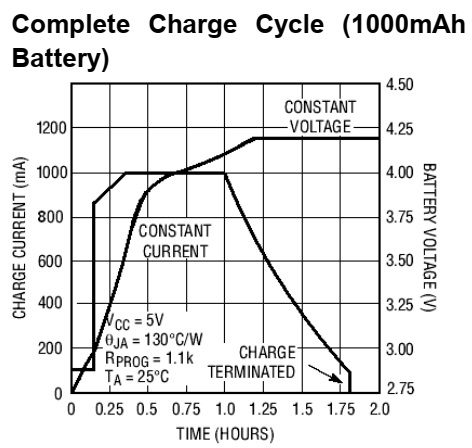
\includegraphics[scale=0.8]{tp4056_complete_charge_cycle.jpg}
    \end{center}
    \caption{TP4056 complete charge cycle}
    \label{fig:tp4056_complete_charge_cycle}
\end{figure}

\subsection{Battery protection}
To protect lithium-ion/polymer battery from damage or degrading the lifetime due to overcharge, overdischarge, and/or overcurrent, a simple battery protection circuit is designed with the use of a DW01A IC and a dual N-channel power MOSFET (FS8205A). The principle of battery protection circuit is shown in figure \ref{fig:dw01a_typical_use}.
\begin{figure}[H]
    \begin{center}
        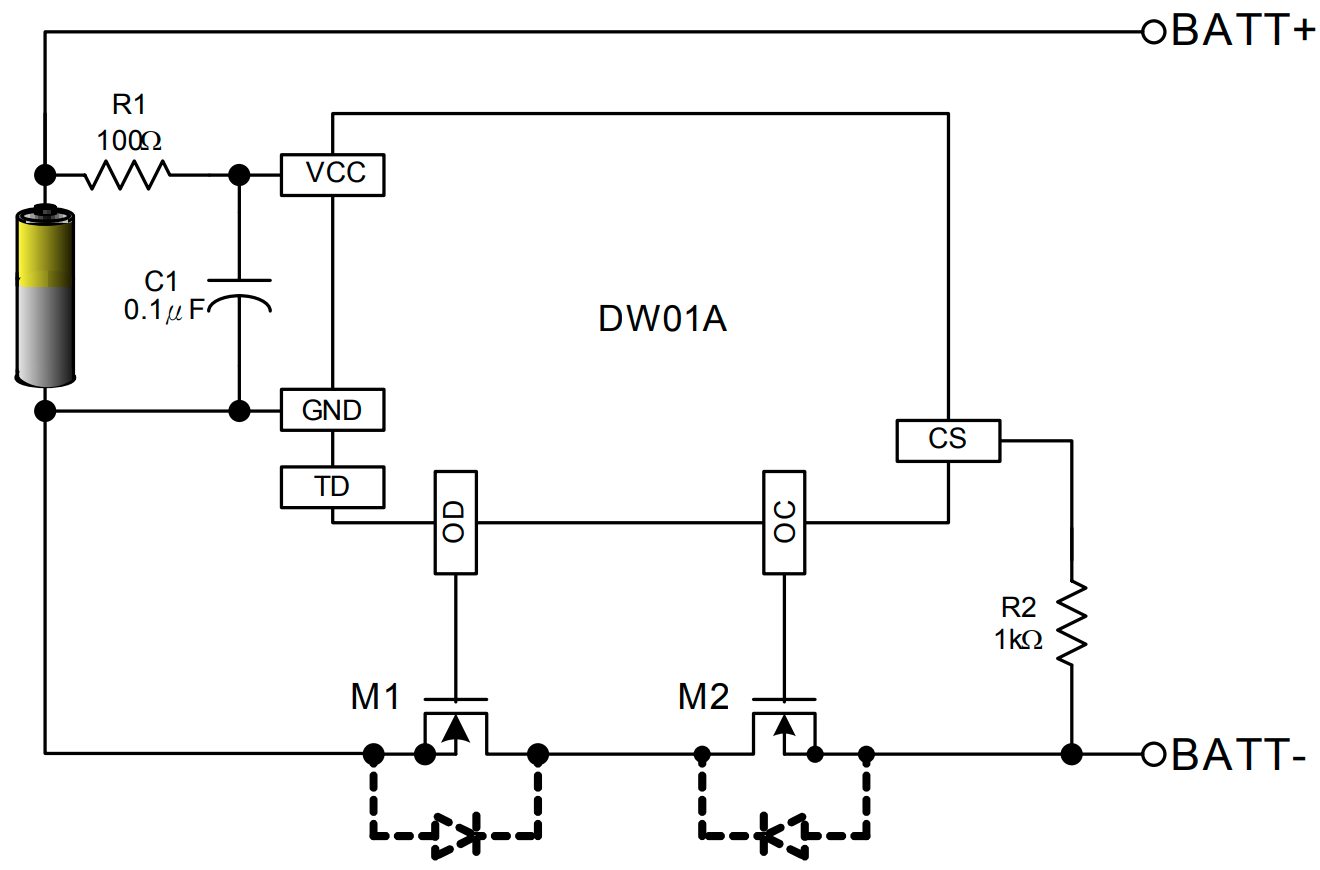
\includegraphics[width=0.7\textwidth]{dw01a_typical_use.png}
    \end{center}
    \caption{DW01A Typical Application Circuit}
    \label{fig:dw01a_typical_use}
\end{figure}
In the DW01A, OC pin is used for charge control and OD pin is used for discharge control.
\subsubsection{Overvoltage charge detection}
This function is used to monitor the charger voltage between $BATT+$ and $BATT-$, when this voltage exceeds overcharge protection voltage ($V_{OCP} = 4.3V$) for the overcharge detection delay time ($T_{OC} = 80ms$) or longer,  the DW01A turns off the charging MOSFET (M2). When this voltage drops below the overcharge release voltage ($V_{OCR} = 4.1V$), it then turns on charging MOSFET (M2).

\subsubsection{Overvoltage discharge detection}
If the battery voltage is less than the overdischarge protection voltage ($V_{ODP} = 2.4V$) during discharging status for the overdischarge detection delay time ($T_{OD} = 40ms$) or longer, the DW01A turns off the discharging MOSFET (M1) to stop discharging. When this voltage rises above the overdischarge release voltage ($V_{ODR} = 3.0V$), it then turns on discharging MOSFET (M1).

\subsubsection{Discharge overcurrent and short-circuit detection}
The CS pin (current sense pin) is used to detect the overcurrent condition. When the voltage at CS pin ($V_{CS}$) is greater than the overcurrent protection voltage ($V_{OIP} = 0.15V$) or the short current protection Voltage ($V_{SIP} = 1.2V$), DW01A turns off the discharging MOSFET (M1). It then turns on discharging MOSFET when $V_{CS}$ drops below the thresholds.

\section{Voltage step down converter}
In this thesis, a switching power supply is used instead of a linear one to increase the power efficiency. The dedicated PWM step-down DC/DC converter IC (RT8059) is able to delivery 1A output current over a wide input voltage range from 2.8V to 5V as provided by the battery. Figure \ref{fig:voltage_set_down_converter} is the schematic for the buck circuit.
\begin{figure}[H]
    \begin{center}
        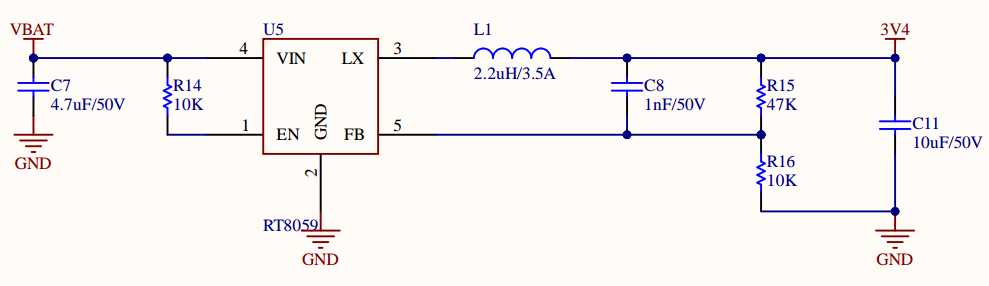
\includegraphics[width=1\textwidth]{voltage_set_down_converter.png}
    \end{center}
    \caption{Voltage set down converter}
    \label{fig:voltage_set_down_converter}
\end{figure}
\subsection{Buck converter}
A buck converter (step-down converter) is a DC-to-DC power converter which steps down voltage (while stepping up current) from its input (supply) to its output (load).

\begin{figure}[H]
    \begin{center}
        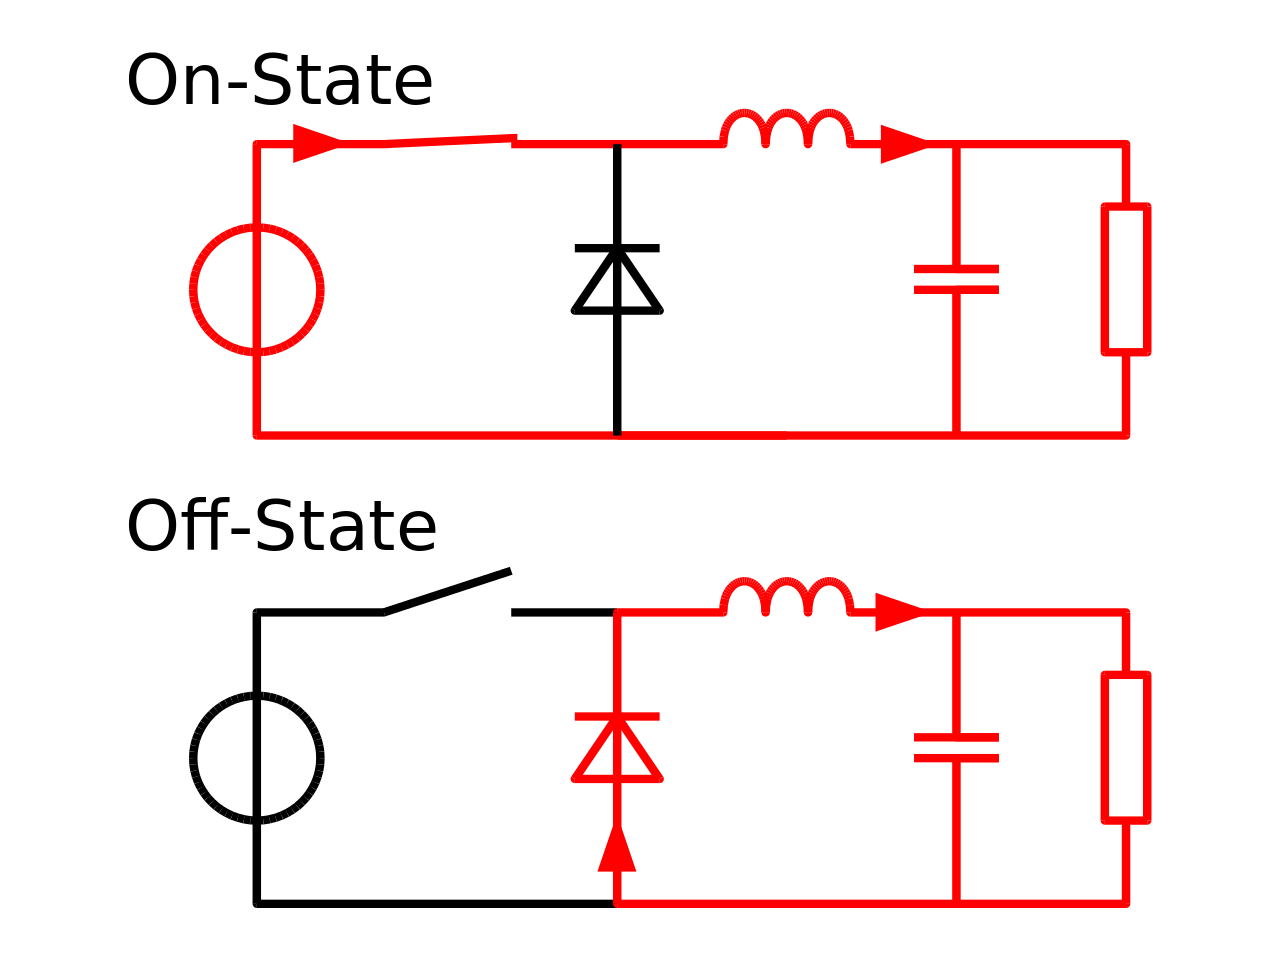
\includegraphics[width=0.5\textwidth]{buck_converter.png}
    \end{center}
    \caption{The two circuit configurations of a buck converter}
    \label{fig:buck_converter}
\end{figure}

The relation between current and voltage of the inductor may be the best explanation to understand the conceptual model of the buck converter. In the beginning, the switch is open (off-state) and the current in the circuit is zero. When the switch is first closed (on-state), the current will begin to increase. In response to the changing current, the inductor will produce an opposing voltage across its terminals. This voltage drop counteracts the voltage of the source and therefore reduces the net voltage across the load. Over time, the voltage across the inductor decreases as the rate of change of current decreases, leading to an increase of the voltage at the load. During this time, energy in the form of a magnetic field is stored in the inductor. If the switch is opened while the current is still changing, then there will always be a voltage drop across the inductor, so the net voltage at the load will always be less than the input voltage source. If the switch is opened again (off-state), the current will decrease since the voltage source is removed from the circuit. The decreasing current will produce a voltage drop across the inductor (opposite to the drop at on-state). Now, the inductor becomes a current source. The current flow through the load is supported by the stored energy in the inductor's magnetic field. During the off-state, the inductor is discharging its stored energy into the rest of the circuit. The charge-discharge process of the inductor results in a smaller average voltage across the load compared with the input voltage.

\subsection{Buck converter in action}

\subsubsection{Inductor selection}
For a given input and output voltage, the inductor value
and operating frequency determine the ripple current. The
ripple current $\Delta I_{L}$ increases with higher $V_{IN}$ and decreases with higher inductance as shown in equation \ref{eqn:riple_current_vs_in_out_inductance}.
Having a lower ripple current reduces the ESR losses in
the output capacitors and the output voltage ripple. At low frequency, the highest efficiency operation requires a large inductor.

\begin{equation}
    \Delta I_{L} = \frac{V_{OUT}}{f\times L} \left(1 - \frac{V_{OUT}}{V_{IN}}\right)
    \label{eqn:riple_current_vs_in_out_inductance}
\end{equation}

A reasonable starting point for selecting the ripple current
is:
\begin{equation}
    \Delta I_{L-max} = 0.4 I_{max} = 0.4 \times 0.5 = 0.2
\end{equation}

The largest ripple current occurs at the highest $V_{IN}$. To guarantee that the ripple current stays below a specified maximum, the inductor value should be chosen according to equation \ref{eqn:riple_current_inductor_condition}.
\begin{equation}
    \begin{split}
        L &\geq \frac{V_{OUT}}{f\Delta I_{L-max}} \left( 1 - \frac{V_{OUT}}{V_{IN-max}}\right)  \\
        &= \frac{3.42}{1.5Mhz \times 0.2} \left( 1 - \frac{3.42}{4.2}\right) \\
        &= 2.1 \times 10^{-6} = 2.1 \mu H
    \end{split}
    \label{eqn:riple_current_inductor_condition}
\end{equation}
The thesis chooses the value of $2.2uH$ for the inductor. This is the closest value available in the market.

\subsubsection{$C_{IN}$ and $C_{OUT}$ Selection}
The minimum value for the input capacitor ($C_{IN} = 4.7 \mu F$) is given in the datasheet. This minimum value is necessary to stabilize the input voltage due to the peak current requirement of a switching power supply.
The best practice is to use low-equivalent series resistance (ESR) ceramic capacitors. 

Equations \ref{eqn:c_out_selection} can be used to adjust the output capacitor values for a desired output voltage ripple:
\begin{equation}
    \begin{split}
        C_{OUT-min} &= \frac{\Delta I_{L}}{8f\Delta V_{OUT}} \\
        &= \frac{\Delta I_{L}}{8f \times 0.1V_{OUT-max}} \\
        &= \frac{0.2}{8 \times 1.5Mhz \times 0.1 \times 3.42} \\
        &= 0.05 \mu F
    \end{split}
    \label{eqn:c_out_selection}
\end{equation}

The value of $C_{OUT} = 10\mu F$ is chosen for this thesis.

\subsubsection{Output voltage setting}
The resistive voltage divider allows the FB pin to sense a fraction of the output voltage as shown in figure \ref{fig:rt8049_setting_output_voltage}.
\begin{figure}[H]
    \begin{center}
        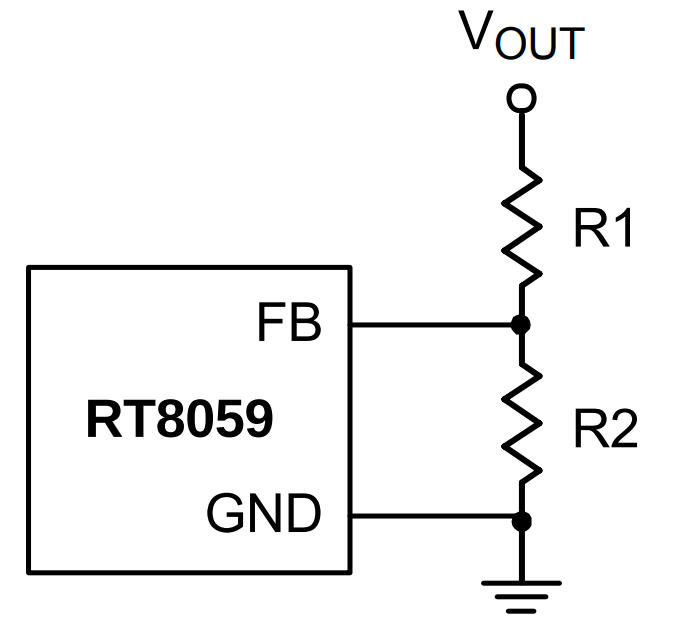
\includegraphics[width=0.3\textwidth]{rt8049_setting_output_voltage.png}
    \end{center}
    \caption{Setting Output Voltage}
    \label{fig:rt8049_setting_output_voltage}
\end{figure}

For adjustable voltage mode, the output voltage is set by an external resistive voltage divider according to equation \ref{eqn:rt8049_voltage_devider}.
\begin{equation}
    V_{OUT} = V_{REF} (1 + \frac{R15}{R16}) = 0.6 (1 + \frac{47}{10}) = 3.42V
    \label{eqn:rt8049_voltage_devider}
\end{equation}
where $V_{REF} = 0.6V$ (typ.) is the internal reference voltage.

\section{Result}
Figure \ref{fig:rtls_anchor_hw_upper} and \ref{fig:rtls_anchor_hw_lower} show the RTLS board designed with Altium Designer. The PDF exported from Altium for hardware design of RTLS anchor board is provided in appendix \ref{appendix:rtls_anchor_board}. In addition, the Solidwork-based design for the enclosure of the RTLS anchor is also given in appendix \ref{appendix:rtls_anchor_enclosure}.
\begin{figure}[H]
    \begin{center}
        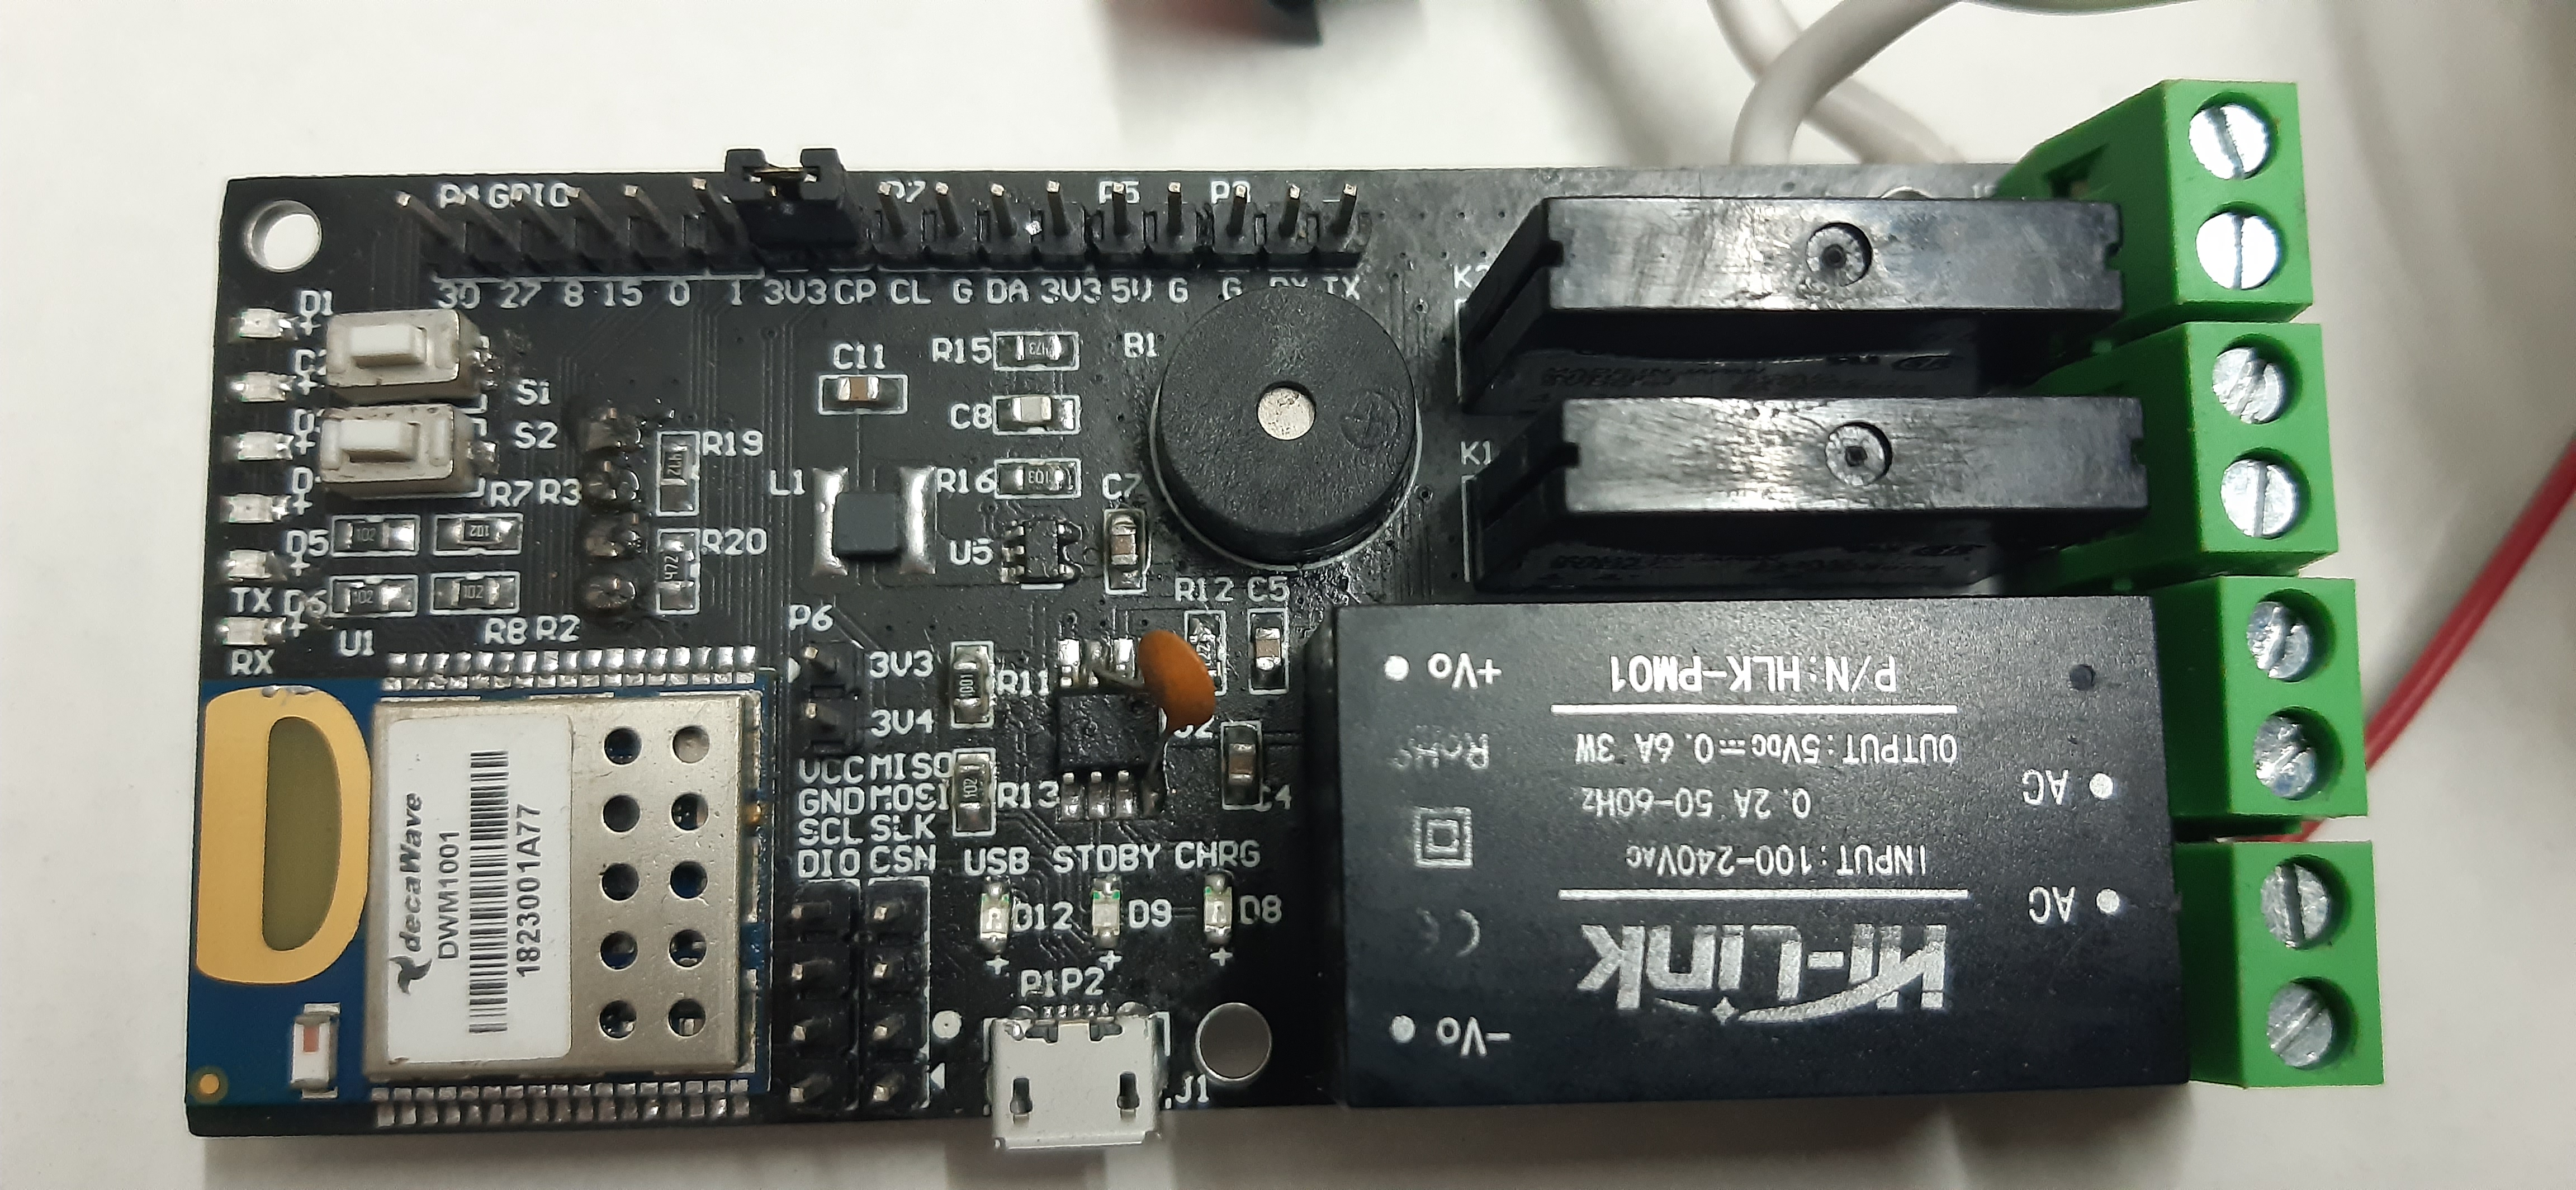
\includegraphics[width=0.9\textwidth]{rtls_anchor_hw_upper.jpg}
    \end{center}
    \caption{RTLS anchor board upper face}
    \label{fig:rtls_anchor_hw_upper}
\end{figure}

\begin{figure}[H]
    \begin{center}
        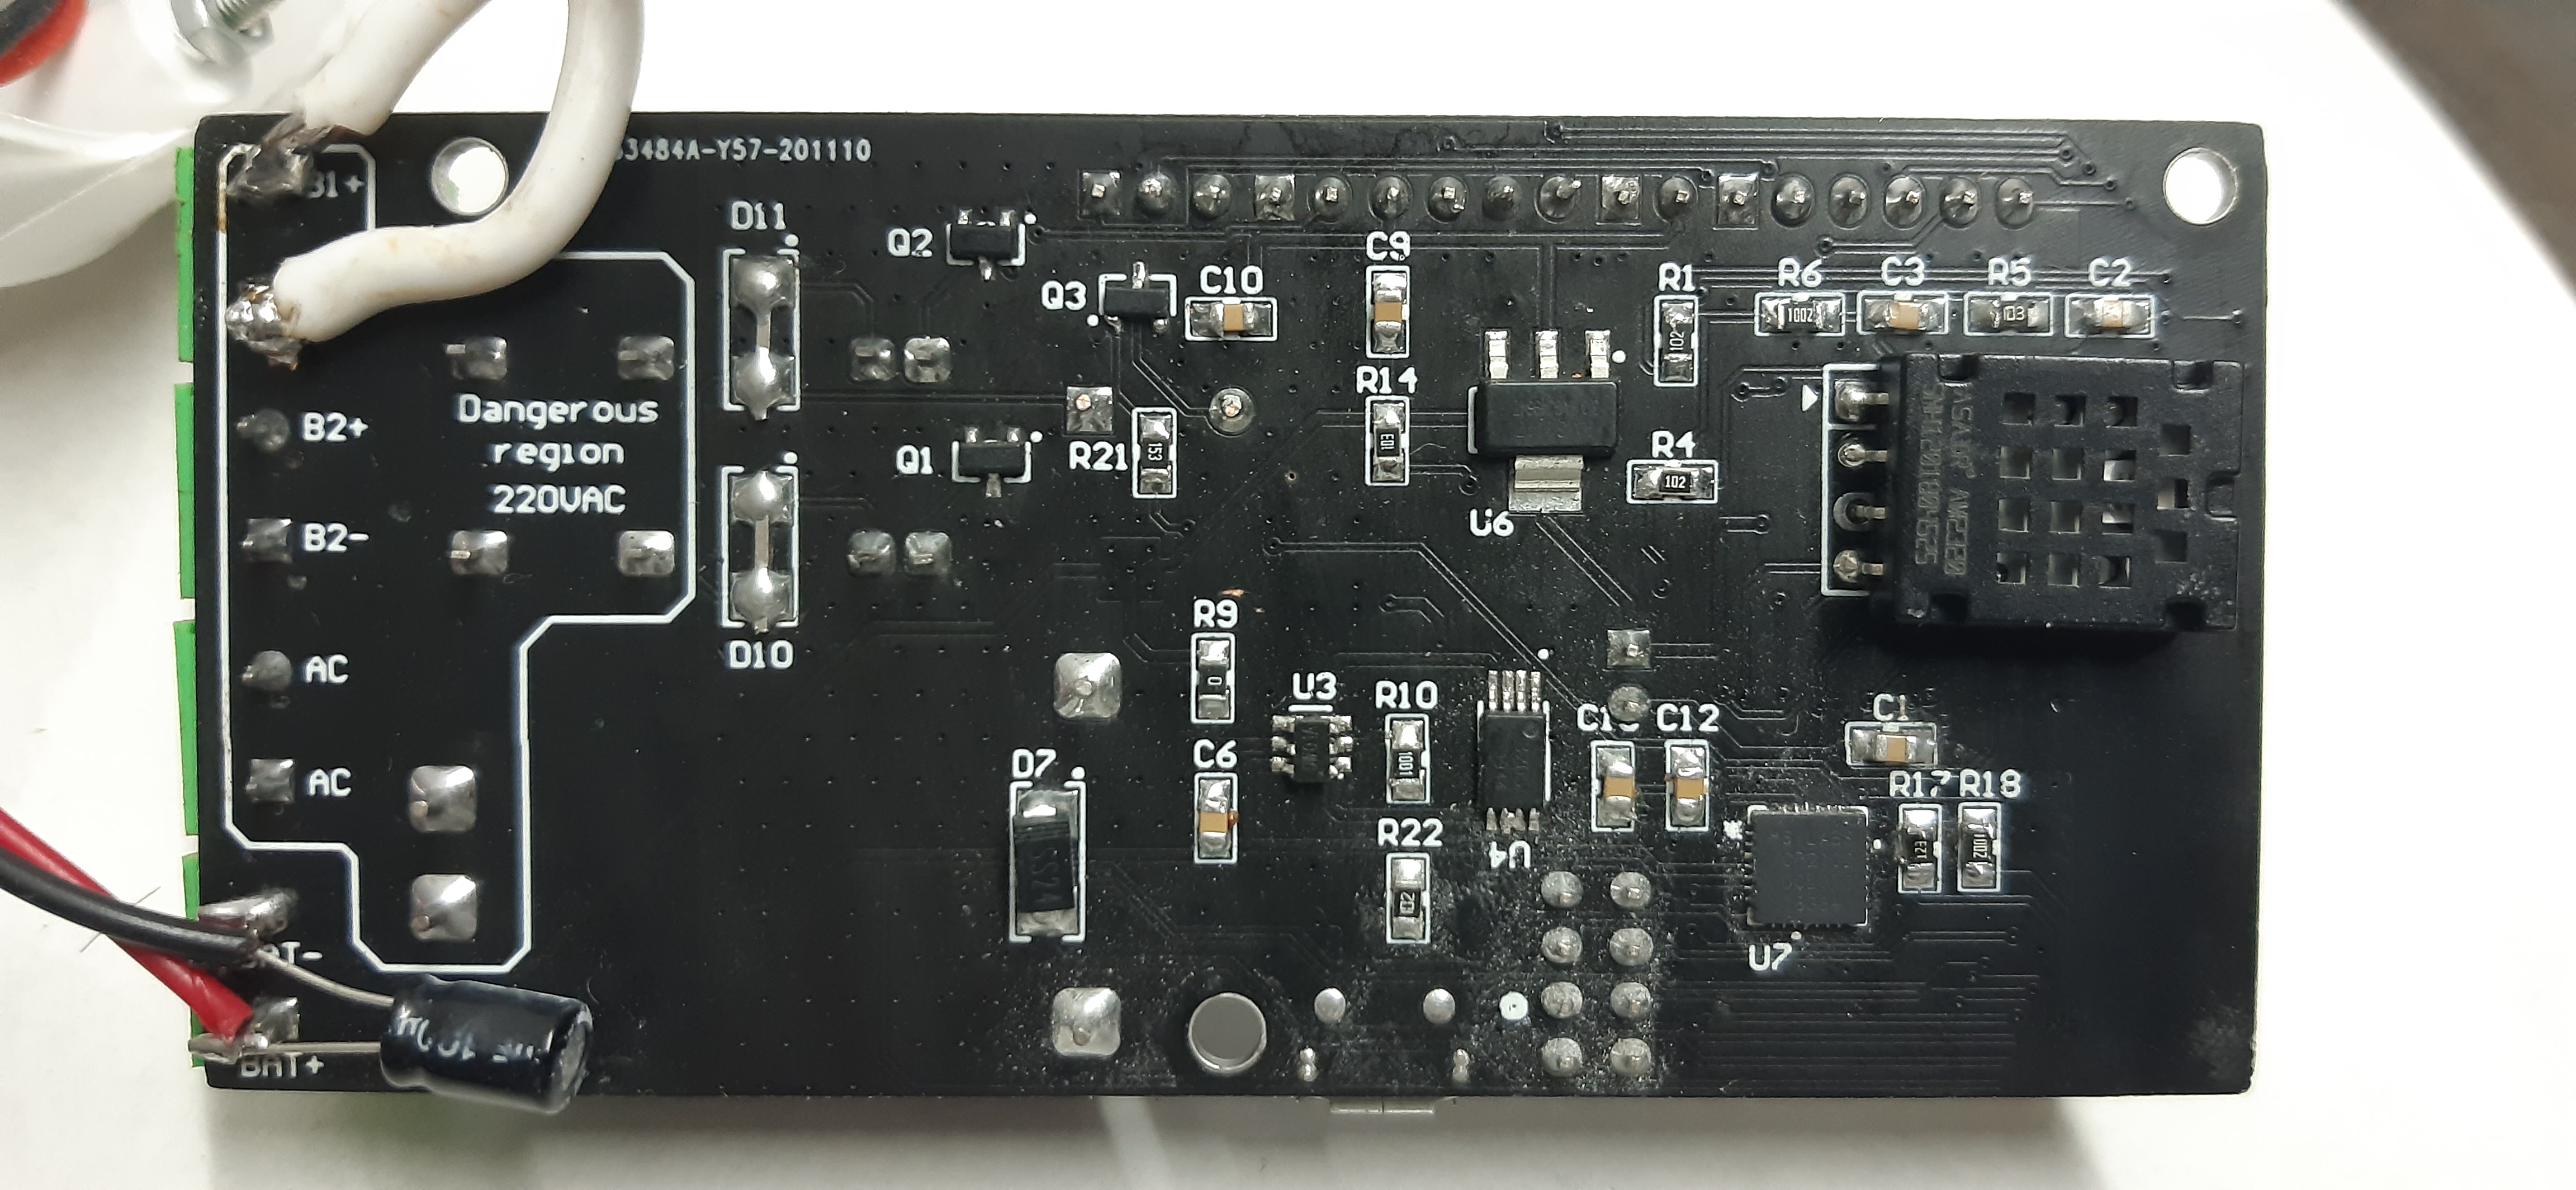
\includegraphics[width=0.9\textwidth]{rtls_anchor_hw_lower.jpg}
    \end{center}
    \caption{RTLS anchor board lower face}
    \label{fig:rtls_anchor_hw_lower}
\end{figure}

\end{document}